\chapter{Introduction}
\label{chapter:Introduction}

For robots to make a smooth ingress into dynamic human environments like home and office, they need to be able to close the \emph{perceive-action-learning} loop \citep{Marc2016}. 
Essentially these domestic service robots should perceive the environment, interact with the environment, learn from experiences and repeat. 
The robot interacts with the environment by choosing a sequence of low-level actions. 
For example, lets take the high-level task of ``making coffee". This will require the following actions to be executed sequentially: locate coffee machine, locate coffee pad, locate a cup, place coffee pad in coffee machine, place cup in coffee machine and start coffee machine. 
However, for executing some of the actions like locating the coffee machine, locating the coffee pads and locating the cup the robot needs to have prior knowledge about their possible locations. Such knowledge about the environment and user preferences can be represented as qualitative models. However, this is cumbersome. An alternative solution can be to learn such knowledge from past observations. The goal of this thesis is to enable domestic service robots to gain knowledge about common behaviours and preferences of the user in a non-intrusive manner. Specifically, we address how Bayesian methods can be used to provide a flexible and computationally efficient structure for acquiring knowledge using limited spatio-temporal information collected by domestic service robots.

Domestic service robots need to have the ability to automatically and quickly adapt to a new environment. Imagine if the robot could learn how the user arranges the breakfast table by looking at the data from previous days. Robots can observe the user's lifestyle and provide small insights which even the user does not notice. The robots can pass along helpful information to the users, like observing their sleep habits and telling them when they are not having adequate sleep. By learning how the user interacts with their homes and how they live their lives, robots will be able to provide better services to their users. 
\begin{figure}[htp]
\centering
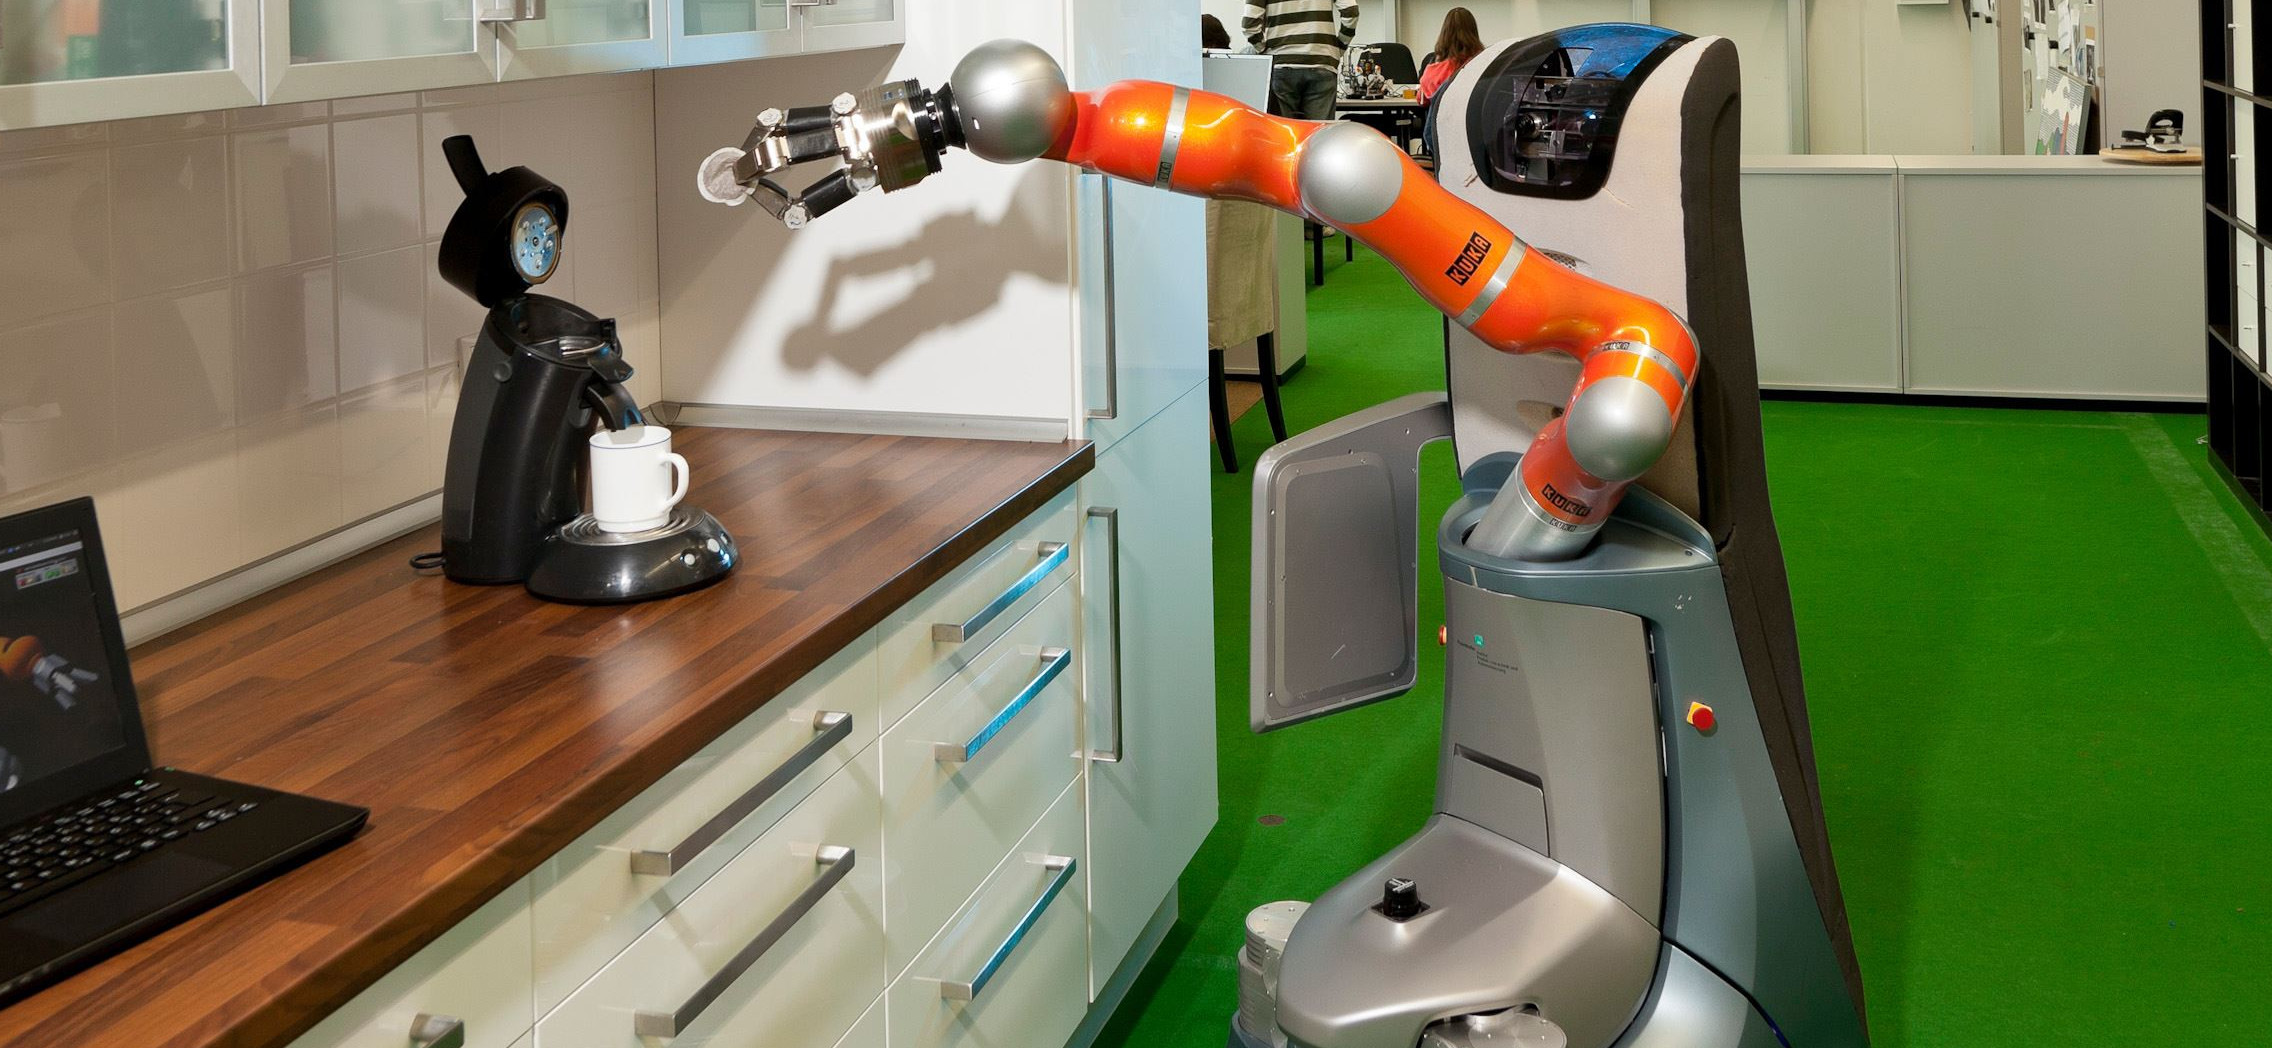
\includegraphics[width=\textwidth]{images/coffee.jpg}
\caption{Illustrative example of a robot making coffee \citep{bitbotsfb}}
\label{}
\end{figure}

To illustrate the relevance of the topics presented in this thesis, we motivate our work using a typical task of a domestic service robot.   We revisit the task of ``making coffee" for the user, which requires the robot to locate the coffee cup of the user first, make coffee and then to locate the user, for delivering the coffee to him. To begin the search for the coffee cup, it would help the robot to have some prior knowledge about the user's habits; in particular the typical locations where he keeps his cup. This enables the robot to funnel its search for the object from a large number of locations to the most probable ones. Once the coffee is made the robot needs to reason about where it can currently find the user for delivering it to him. This in turn, requires the robot to have knowledge about the likely locations of the user at that time.

\begin{figure}[htp]
\centering
\begin{subfigure}{\textwidth}
  \centering
  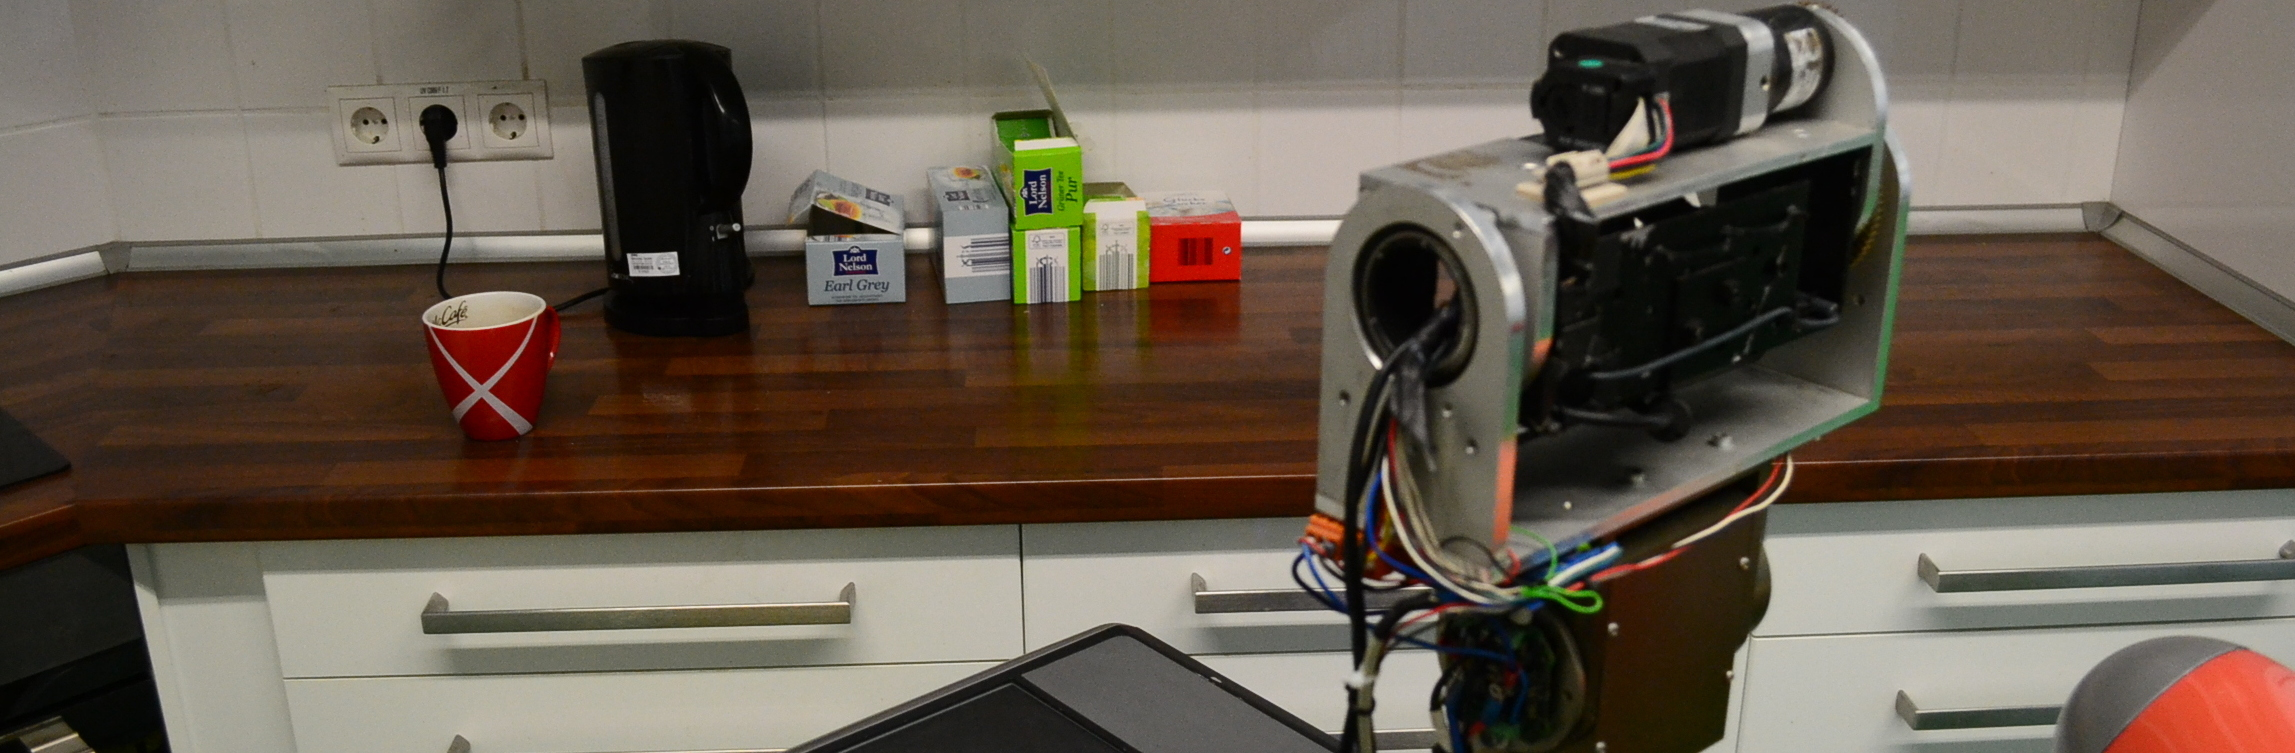
\includegraphics[width=\linewidth]{images/introduction.jpg}
\end{subfigure}%
\\[0.5ex] 
\begin{subfigure}{.243\textwidth}
  \centering
  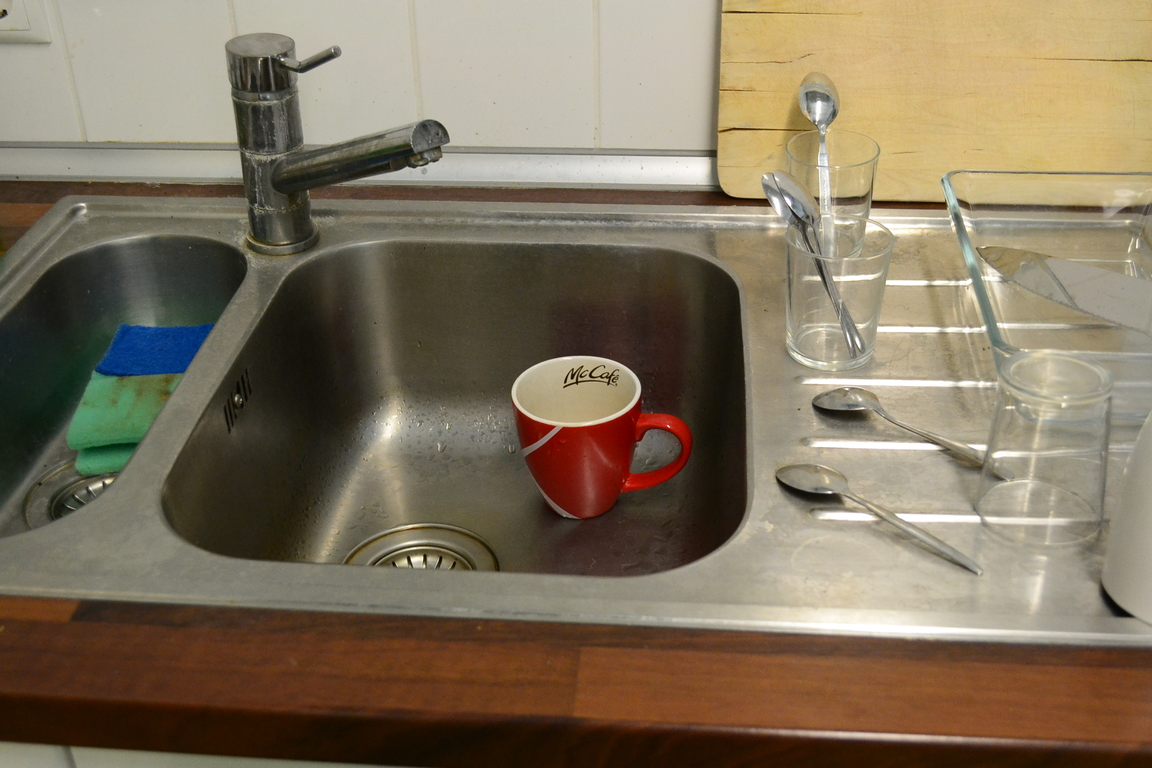
\includegraphics[width=\linewidth]{images/cup_sink.jpg}
  \caption{cup in sink}
\end{subfigure}
\begin{subfigure}{.243\textwidth}
  \centering
  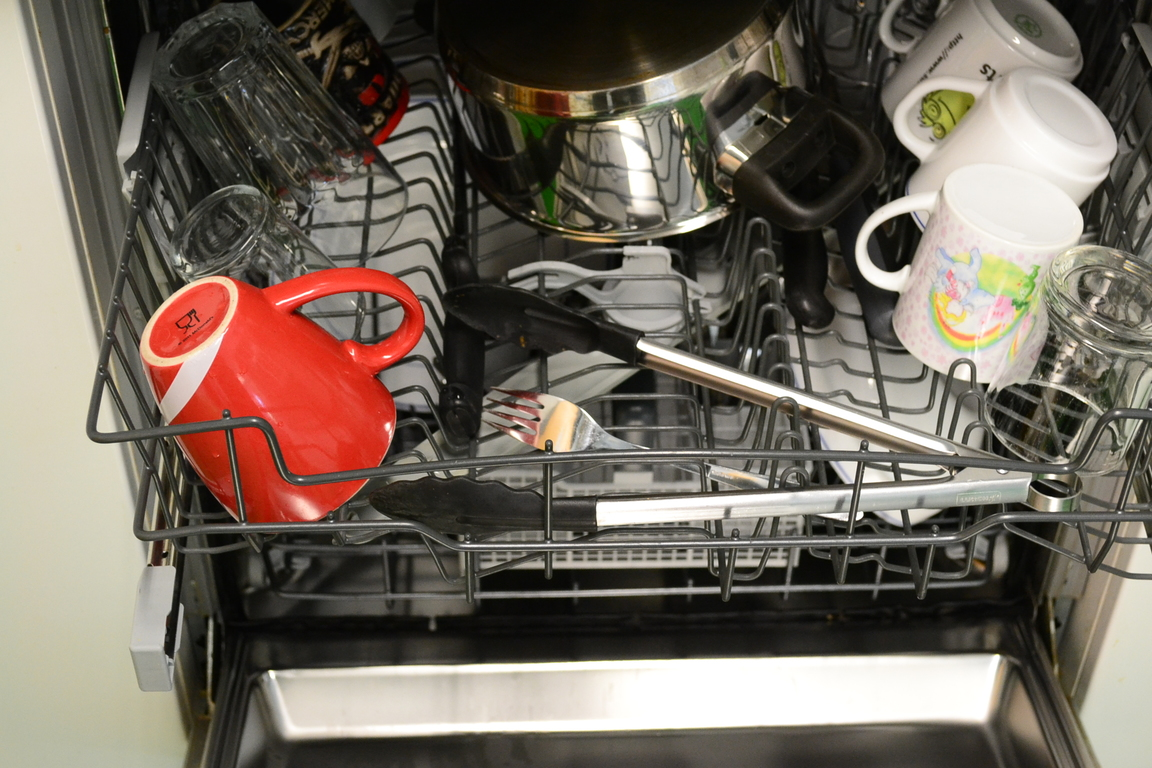
\includegraphics[width=\linewidth]{images/cup_dishwasher.jpg}
    \caption{cup in dishwasher}
\end{subfigure}
\begin{subfigure}{.243\textwidth}
  \centering
  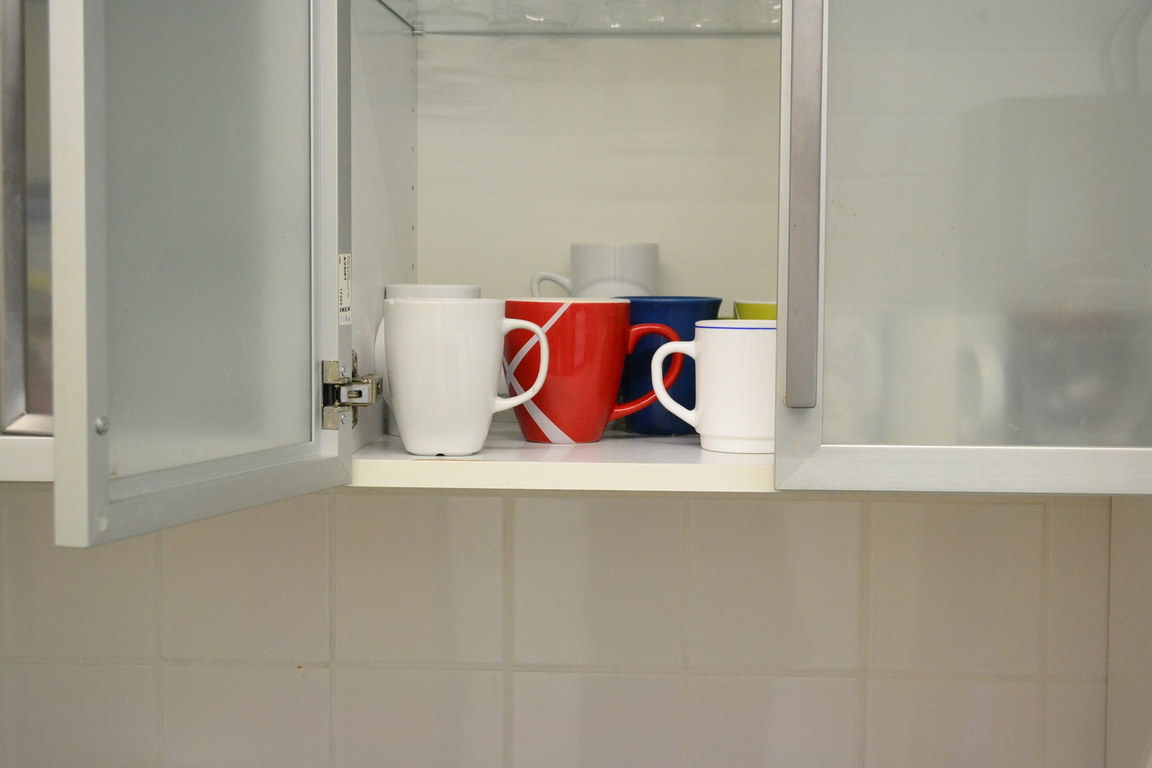
\includegraphics[width=\linewidth]{images/cup_cupboard.jpg}
    \caption{cup in cupboard}
\end{subfigure}
\begin{subfigure}{.243\textwidth}
  \centering
  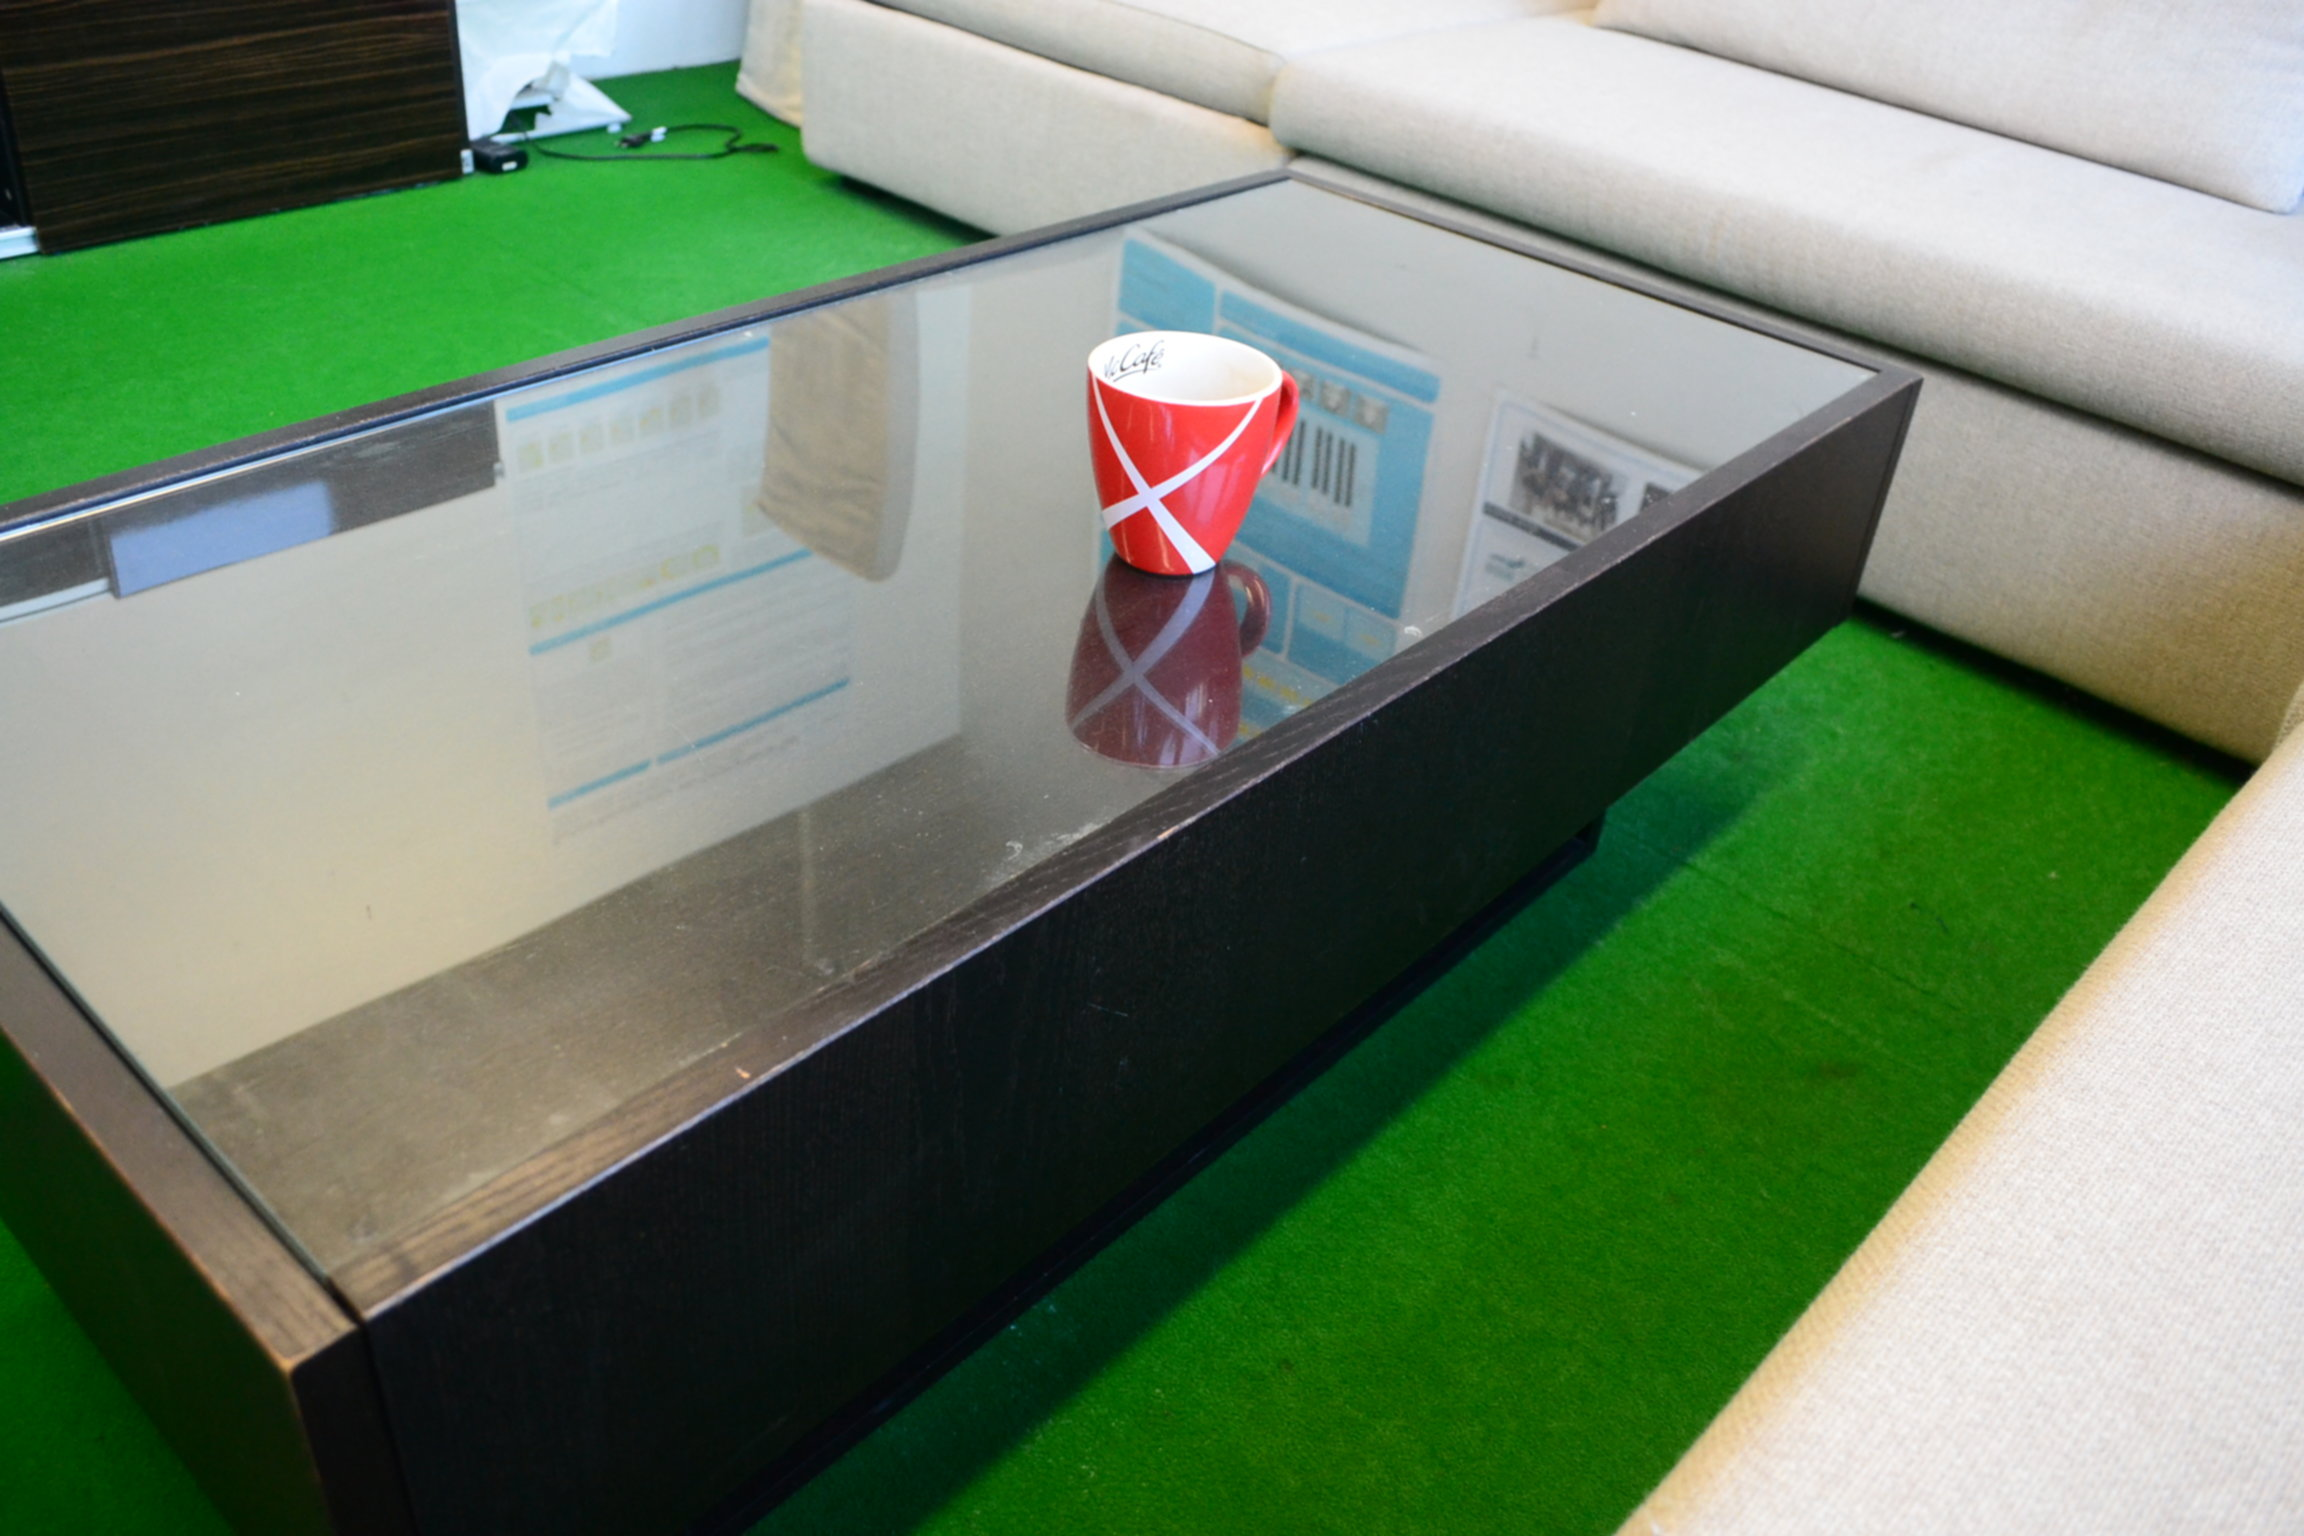
\includegraphics[width=\linewidth]{images/cup_on_table.jpg}
    \caption{cup on table}
\end{subfigure}

\caption[Illustrative example of robot information collection]{Illustrative example of the robot making a record of location of cup}
\end{figure}

\FloatBarrier
This motivating example leads us to the three research topics in knowledge acquisition we address in this thesis:
\begin{enumerate}
	\item How can a domestic service robot acquire knowledge about the user preferences in placing objects in the environment?
	\item How can a domestic service robot acquire knowledge about the user location preferences?
	\item How can a domestic service robot acquire the above knowledge using small amounts of information?
\end{enumerate}


Domestic service robots, while interacting with the user and environment, produce information which are discarded after being processed in perception, actuation, or decision making. \cite{niemueller2012generic} proposed an approach of storing this information in a database and querying the memory for meaningful insights. 
The domestic robot will continuously record sightings of objects and persons with position and time in a database to form a spatio-temporal robot memory.
Information thus collected in the robot memory can be used to build a model of the user preferences. These models represent the internal beliefs of the robot about the user preferences. These models acquire knowledge about the user preferences. But in order to adapt quickly the robot needs to able to extract valuable knowledge from a small amount of information, i.e., the learning algorithms need to be data efficient. There are many approaches that demonstrate that data-efficient machine learning is possible, including methods like: explicit domain knowledge modelling, exploiting structural knowledge of data, bootstrapping and data augmentation, semi-supervised learning, transfer learning, active learning and Bayesian optimization, non-parametric methods, one-shot learning and Bayesian deep learning \citep{MarcICML2016}. Bayesian probabilistic formulation of the model is an approach for data-efficient machine learning \cite{Bishop20120222}.


This thesis provides Bayesian probabilistic techniques that enable a domestic service robot
\begin{itemize}
	\item to learn the user preference model in object placement. 
	\item to learn the user's location preference model.
	\item to learn with limited information.
\end{itemize}


All of our approaches are based on state-of-the art Bayesian learning techniques such as graphical models and probabilistic programming. The probabilistic formulation is used to represent the state of its knowledge about the user's preferences. In a set of experiments on real-world and simulated datasets we show that our approaches are able to successfully extract knowledge about user's preferences in location and object placement from observations made by a domestic service robot. Furthermore, we also demonstrate that the acquired knowledge can be utilized in smart decision making frameworks which can accommodate vision recognition faults. We hope that our approaches will set up service robots into the existing household by knowing what and who are there and adapting to them. These service robots will grow and change with the users, with a greater awareness of the world around them.

